\section{March 4, 2021} 
\subsection{The tangential connection in $S^2$}
Consider $S^2 \subseteq \R^3$, with the angle $\theta$ sweeping across the equator and $\varphi $ measuring longitudinal distance from the north pole. So $\Sigma(\varphi ,\theta)=(\sin \varphi  \cos \theta, \sin \varphi  \sin \theta, \cos \varphi ).$ In terms of coordinates, say $x^1=\varphi $ and $x^2=\theta$. We know $\partial _{\varphi }\Sigma=(\cos \varphi  \cos \theta, \cos \varphi  \sin \theta, - \sin \varphi )=e_1$, $\partial _{\theta}\Sigma=(-\sin \varphi  \sin \theta, \sin \varphi  \cos \theta, 0)=e_2$. So $g_{11}=1,g_{12}=0,g_{22}=\sin ^2 \varphi $. We want to compute $\nabla _{e_1}e_1,\nabla _{e_1}e_2,\nabla _{e_2}e_1,\nabla _{e_2}e_2$. For tangential connections, we use the connection on the big space $\R^3$, which is trivial. We have
    \begin{alignat*}{2} 
        &\overline{\nabla} _{e_1}e_1=(-\sin \varphi  \cos \theta,-\sin \varphi  \cos \theta, -\cos \varphi )=-\Sigma,\quad &&\overline{ \nabla }_{e_1}e_2=(-\cos \varphi \sin\theta, \cos \varphi  \cos \theta,0)=\cot \varphi e_2,\\
        &\overline{\nabla }_{e_2}e_1=(- \cos \varphi  \sin \theta, \cos \varphi  \cos \theta,0)=\cot \varphi  e_2,&&\overline{\nabla}_{e_2}e_2=(-\sin \varphi  \cos \theta,-\sin \varphi  \sin \theta,0)=-\sin \varphi  \cos \varphi  e_1.
    \end{alignat*}
    To calculate $\overline{\nabla}_{e_1}e_2,$ note that $\overline{\nabla}_{e_1}e_2\perp e_1$. So the projection is some multiple of $e_2$: to figure out what the multiple is, we want to calculate 
    \[
    \pi_{e_2}(\overline{\nabla}_{e_1}e_2)=\frac{(\overline{\nabla}_{e_1}e_2)\cdot e_2}{e_2\cdot e_2}e_2=\frac{ \sin \varphi  \cos \varphi }{\sin ^2 \varphi }e_2=\frac{\cos \varphi }{\sin \varphi }e_2=\cot \varphi e_2.
\] Why are we just taking derivatives with respect to $\varphi $ and $\theta$ to calculate the $\nabla$'s? In $\R^3$, $(\overline{\nabla}_v w)^j =v(w^j )=v^i \partial _i w^j $. Since $e_1=\partial _{\varphi },e_2=\partial _{\theta}$, we have $\overline{\nabla}_{e_1}=\partial _{\varphi },\, \overline{\nabla}_{e_2}\partial _{\theta}$. After doing these calculations, we just project down. Given an orthonormal frame $\{e_i \} $, and a vector $v$, then \[
\pi_{\text{plane} }v= \frac{v\cdot e_1}{e_1\cdot e_1}e_1+\frac{v\cdot e_2}{e_2\cdot e_2}e_2=\frac{v\cdot e_i }{e_i \cdot e_i }e_i \ \ \text{\small(implicit sum).}
\] The final component $\overline{\nabla}_{e_2}e_2$ is the tricky one. It looks sort of like the position, but it has no third component. It's not entirely pointing in the normal direction, it has a tangential component. Since $\overline{\nabla}_{e_2}e_2\perp e_2$, and $\overline{\nabla}_{e_2}e_2\cdot e_1=-\sin \varphi  \cos \varphi ,\ e_1\cdot e_1=1$, we conclude $\overline{\nabla}_{e_2}e_2=-\sin \varphi  \cos \varphi  e_1$. Finally, we conclude that 
    \begin{alignat*}{2} 
        &\nabla _{e_1}e_1=0,\quad &&\nabla _{e_1}e_2=\cot \varphi e_2,\\
        &\nabla _{e_2}e_1=\cot \varphi  e_2,\quad&&\nabla_{e_2}e_2= - \sin \varphi  \cos \varphi  e_1.
    \end{alignat*}
    Now that we know this, we can take the derivative of \emph{any} vector field on $S^2$ with respect to \emph{any} other vector field on $S^2$, since we've worked out what all the Christoffel symbols are. How do we geometrically interpret our results? 

    \begin{figure}[H]
    \centering
     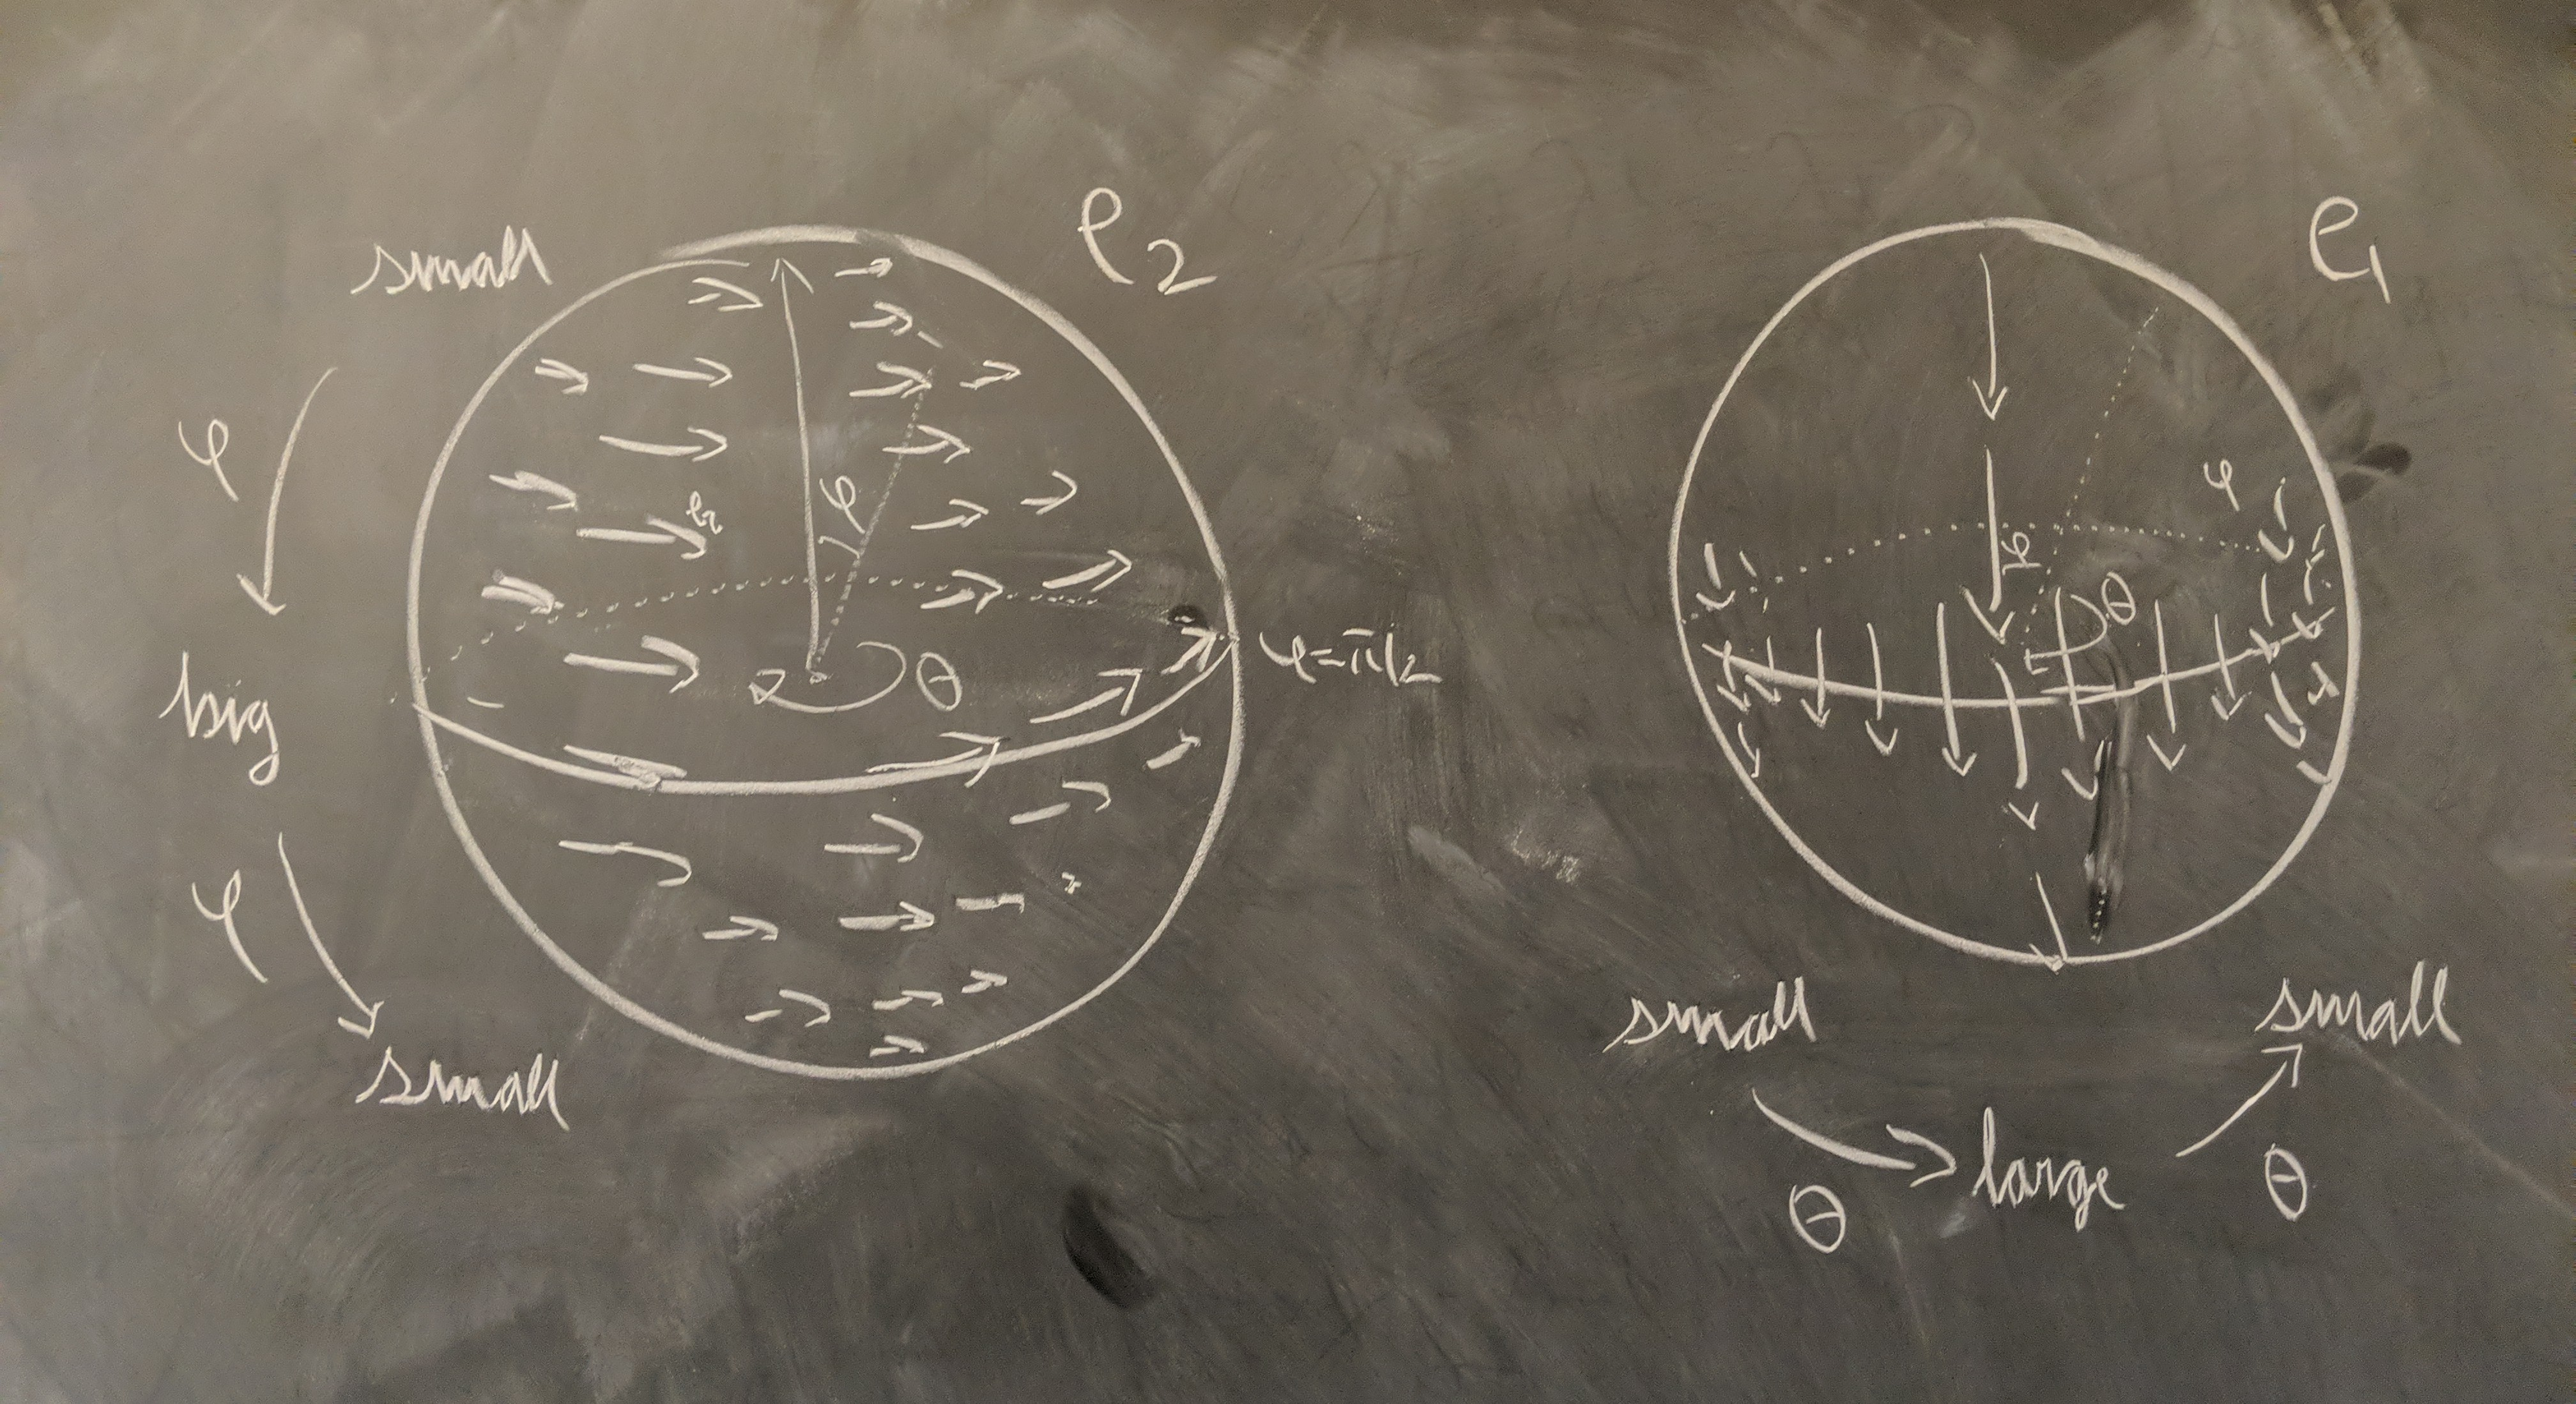
\includegraphics[width=0.6\linewidth]{figures/rgeo_lec12.1.jpg}
    \end{figure}

    The vector field $e_2$ is small at the poles and grows larger as it goes south from the north pole (moving in the $\varphi $ direction), then starts to decrease as it approaches the south pole. A similar thing happens for $e_1$, which is large at the great circle connecting the poles, but gets smaller as you go farther out east or west (in the $\theta$ direction). The precise coefficient $\cot \varphi $ is a calculation, but this is the general idea. 

    Now that we've developed the theory of connections, let's return to the geodesic.
\begin{definition}[]
    A \textbf{geodesic} with respect to a covariant derivative $\nabla$ is a curve satisfying $\nabla _{\dot x}\dot x=0$. In terms of coordinates, we have $\ddot x^k+\Gamma _{ij}^k \dot x^i \dot x^j =0$.
\end{definition} Is this equivalent to the other definitions of a geodesic? It turns out there is a certain connection that satisfies this, the \emph{Levi-Civita connection}. 

\subsection{The fundamental theorem of Riemannian geometry}
Let's recall some properties that connections can have.
\begin{itemize}
    \item A connection is \textbf{metric} if $\nabla g=0$, which is equivalent to $X(g(Y,Z))=g(\nabla_XY,Z)+g(Y,\nabla_XZ)$. In particular, for $X=e_i ,Y=e_j ,Z=e_k$, we have $\partial _i g_{jk}=g(\nabla _i e_j ,e_k)+g(e_j ,\nabla _i e_k)=g(\Gamma _{ij}^{\ell}e_{\ell},e_k)+g(e_j ,\Gamma _{ik}^me_m)=\Gamma _{ij}^{\ell}g_{\ell k}+\Gamma _{ik}^m g_{jm}$, then set $\Gamma _{ij}^{\ell} g_{\ell k}=\Gamma _{ijk}$ and $\Gamma _{ik}^mg_{jm}=\Gamma _{ikj}$. In short, $\boxed{ \partial _i g_{jk}=\Gamma _{ijk}+\Gamma _{ikj}.}$ 
\end{itemize}
Note that our tangential connection $\nabla=\pi(\overline{\nabla})$ on $S^2$ is metric. The question is, does $X(g(Y,Z))=g(\nabla_XY,Z)+g(Y,\nabla_XZ)$? We have $g(\nabla_XY,Z)+g(Y,\nabla_XZ)= g(\pi(\overline{\nabla}_XY),Z)+g(Y,\pi(\overline{\nabla}_XZ))$: the difference between $\nabla$ and $\overline{\nabla}$ of something results in something in the perpendicular direction. Then taking the inner product of something in the perpendicular direction with the tangent direction gives zero, so $g(\pi(\overline{\nabla}_XY),Z)+g(Y,\pi(\overline{\nabla}_XZ))=g(\overline{\nabla}_XY,Z)+g(Y,\overline{\nabla}_XZ).$ Then since $\overline{\nabla}$ is metric, $\nabla$ must be metric as well.
\begin{itemize}
    \item A connection is \textbf{symmetric} (or \textbf{torsion-free}) if $[X,Y]=\nabla_XY-\nabla_YX$.
\end{itemize}
In $\R^n $ this is true, since we compute the bracket of vector fields is by taking the ordinary derivatives of the coefficients, which is the same as taking covariant derivatives of the coefficients. What does this mean in terms of Christoffel symbols? If $X= \frac{\partial}{\partial x^i },Y=\frac{\partial }{\partial x^j }$, then $[X,Y]=0$. So  $0=\nabla _i e_j -\nabla _j e_i =\Gamma _{ij}^k e_k-\Gamma _{jk}^ke_k$, so $\Gamma _{ij}^k=\Gamma _{ji}^k$. In Euclidian space, both coefficients are zero, so the standard connection is symmetric.

\begin{theorem}\label{symm} 
    If $\overline{\nabla}$ is metric and symmetric, so is the tangential connection $\nabla^T$.
\end{theorem}
\begin{proof}
    We have already shown the metric part of this result. Consider $[X,Y]=\overline{\nabla}_XY -\overline{\nabla}_YX$ by assumption. Then $\pi([X,Y])=\pi(\overline{\nabla}_XY)-\pi(\overline{\nabla}_YX)$. Since $[X,Y]$ is the bracket of two tangent vectors fields and therefore a tangent vector field, applying the \emph{tangential} projection does nothing. Furthermore, $\pi(\overline{\nabla})=\nabla$, so we have $[X,Y]=\nabla_X Y-\nabla_YX$.
\end{proof}
\begin{namedthm}{Fundamental Theorem of Riemannian Geometry} 
    For any Riemannian manifold $(M,g)$, there exists a unique connection that is metric and symmetric. 
\end{namedthm}
\begin{cor}\label{eg} 
    The tangential connection $\nabla^T$ is completely determined by the metric $g$.
\end{cor}
The result of \cref{eg} is strange, since $\nabla^T$ is an \emph{extrinsic} property: it's all about how something is sitting in space, and is \emph{not} preserved by isometries. However, it's determined by an \emph{intrinsic} property, the metric. When Gauss came up with this theorem in the context of surfaces, he called it the \textbf{Theorema Egregium}. Now let's prove our big theorem.

\begin{proof}[Proof of the Fundamental Theorem of Riemannian Geometry]
    Recall that a metric connection implies that $\partial _i g_{jk}=\Gamma _{ijk}+\Gamma _{ikj}$, and a symmetric connection satisfies $\Gamma _{ij}^k=\Gamma _{ji}^k, $ which implies $\Gamma _{ijk}=\Gamma _{jik}$. Then consider
    \begin{align*}
        \partial _i g_{jk}&=\Gamma _{ijk}+\Gamma _{ikj}\\
    +(\partial _j g_{ik}&=\Gamma _{jik}+\Gamma _{jki})\\
    -(\partial _k g_{ij}&=\Gamma _{kij}+\Gamma _{kji}),
    \end{align*} and since $\Gamma _{kij}=\Gamma _{ikj},\Gamma _{kji}=\Gamma _{jki}$, four out of six terms cancel and we are left with 
    \begin{align*}
        \partial _i g_{jk}&+\partial _j g_{ik}-\partial _kg_{ij}=2\Gamma _{ijk} \implies \\
        \Gamma _{ijk}&=\frac{1}{2}\left( \partial _i g_{jk}+\partial _j g_{ik}-\partial _kg_{ij}\right), \\
        \Aboxed{ \Gamma _{ij}^k&=\frac{1}{2}g^{km}(\partial _i g_{jm}+\partial _j g_{im}-\partial _mg_{ij}).}
    \end{align*}
    Here, $g^{km}$ denote the coefficients of the dual metric tensor, or inverse matrix. This connection is called the \textbf{Levi-Civita} connection. We have $\Gamma _{ij}^k$ symmetric since interchanging the roles of $\partial _i g_{jk}$ and $\partial _j g_{ik}$ does nothing (addition is commutative). This is also metric since \[
        \Gamma _{ijk}+\Gamma _{ikj}=\frac{1}{2}\left( \partial _i g_{jk}+\partial _j g_{ik}-\partial _kg_{ij}\right)+\frac{1}{2}\left( \partial _i g_{jk}+\partial _k g_{ij}-\partial _jg_{ik}\right)=\partial _i g_{jk}.\qedhere
    \] 
\end{proof}

\subsection{Computing Christoffel symbols of the Levi-Civita connection}

\begin{example}
    Consider $\R^2$ with polar coordinates $e_1=\partial _r,e_2=\partial _{\theta}$. Our metric is $g_{11}=1,g_{12}=0,g_{22}=r^2$. There are eight $\Gamma _{ij}^k$'s, but only a couple are interesting. We know $\partial_1g_{22}=2r $, while all other derivatives are zero. First, let's compute the $\Gamma _{ijk}$'s. All are zero but $\Gamma _{122}=\frac{1}{2}(\partial_1g_{22}+0-0)=r,\Gamma _{212}=\frac{1}{2}(0+\partial_1g_{22}-0)=r, $ and $\Gamma _{221}=-r$. So
    \begin{align*}
        \Gamma _{11}^1&=0,\\
        \Gamma _{11}^2&=0,\\
        \Gamma _{12}^1&=0,\\
        \Gamma _{12}^2&=\frac{1}{2}g^{2m}(\partial_1g_{2m}+0-0) =\frac{1}{2}g^{22}(\partial_1g_{22})=\frac{1}{2r^2}2r=\frac{1}{r},\\
        \Gamma _{21}^1&=0,\\
        \Gamma _{21}^2&=\Gamma _{12}^2=\frac{1}{r},\\
        \Gamma _{22}^1&=\frac{1}{2}g^{1m}(0+0-\partial_mg_{22}) =-r,\\
        \Gamma _{22}^2&=0.\\
    \end{align*}
\end{example}

\begin{example}
    Let us return to $S^2$. We have $g_{11}=1,g_{12}=0,g_{22}=\sin ^2 \varphi $. The only relevant derivative is $\partial_1g_{22}=2 \sin \varphi  \cos \varphi  $, all other derivatives are zero. Then $\Gamma _{122}=\Gamma _{212}=\frac{1}{2}(\partial_1g_22)=\sin \varphi \cos \varphi  $. Similarly, $\Gamma _{221}=-\sin \varphi  \cos \varphi $. When you raise the indices, you get $\Gamma _{12}^2=\Gamma _{21}^2= \frac{\sin \varphi  \cos \varphi }{\sin ^2 \varphi }=\cot \varphi $, and $\Gamma _{22}^1=-\sin \varphi  \cos \varphi $. This is exactly what we got from our extrinsic calulation at the beginning of lecture!
\end{example}
So we don't need to know how exactly it's sitting in $\R^3$, we only need to know how the metric works. There's a particular space that doesn't sit particularly well in $\R^3$ but for which we understand the metric quite well... the hyperbolic plane! It's not the tangential connection, but the unique symmetric connection instead. The metric on $\H$ is $g_{11}=g_{22}=\frac{1}{y^2}$, and $g_{12}=0$. Once we know what the Christoffel symbols are, we know what a geodesic is!
